\begin{figure}
\centering 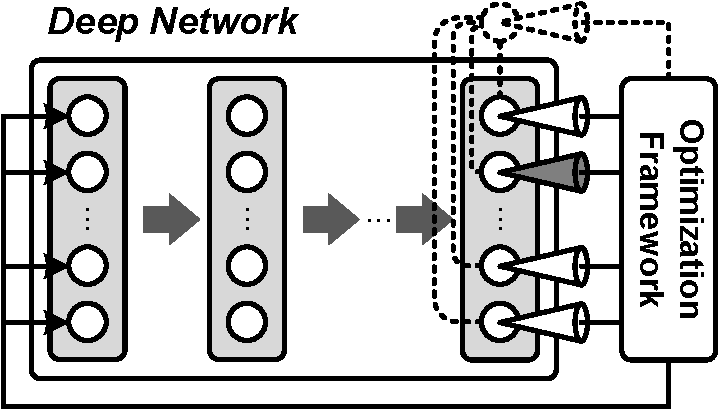
\includegraphics[width=0.5\textwidth]{Figs/concept.pdf} 
\caption{ 
{\bf Schematic of numerical optimization framework.} (A) Here we consider a deep network, which consists of a hierarchical cascade of layers (shaded tall rectangles) of artificial neurons (circles) transform a pixel stimulus $x$ (bottom layer, leftmost) into a high-level feature representation $r$ (top layer, rightmost) suitable for classification.  To study the properties of units within these networks, we employ an optimization framework shown in (B).  The framework consists of a closed-loop algorithm that iteratively measures the response(s) of one or multiple neuron(s), computes the value of a predefined ``fitness'' function, and adaptively generates new stimuli to characterize the target neuron(s).  Different fitness functions allow us to probe different properties of the units (see Eq.~(\ref{eq:O1}--\ref{eq:S2})).
%optimizing the fitness functions defined for different purposes (see Eq.~(\ref{eq:O1}--\ref{eq:S2})); when characterizing multiple neurons for population representation of given optimal or reference stimulus, response of an imaginary neuron (dashed circle) tuned to the given stimulus is optimized (see Eq.~(\ref{eq:O2}, \ref{eq:I2}, \ref{eq:S2})) equivalently.}
\label{fig:concept}
\end{figure}

Figure \ref{fig:concept} illustrates and defines the setup of the closed-loop numerical optimization framework for studying sensory representations encoded within the deep network of interest. The proposed framework consists of two main methods: (1) optimal stimulus search and (2) invariance/selectivity path search, or the first-order and quasi-second-order characterization methods, which equivalently correspond to the linear analysis and low-rank quadratic analysis (i.e.~only eigenvectors of the largest and smallest eigenvalues considered) respectively. Representation $r$, in this work, is equivalent to the response(s) of artificial neuron(s), and is denoted as unit representation (or scalar representation, i.e.~$r \in \mathbb{R}$) when referring to single neurons and population representation (or vector representation, i.e.~$r \in \mathbb{R}^R$) when referring to groups of neurons (with group size $R$). Arguably, for studying both artificial and biological neural networks, the ability to characterize population representations is arguably at leaast as importnat, if not more important than of characterizing unit representations \cite{churchland}. This framework supports characterizing both unit (using Eq.~(\ref{eq:O1}, \ref{eq:I1}, \ref{eq:S1}), though Eq.(\ref{eq:O2}, \ref{eq:I2}, \ref{eq:S2}) can be used as well) and population (using Eq.(\ref{eq:O2}, \ref{eq:I2}, \ref{eq:S2})) representations in a unified way.

Our framework treats networks as non-analytical black boxes: it makes no assumption about network structure or properties (e.g. we do not assume an analytical gradient is available, even though such gradients are available for many kinds of artificial networks). We made this strategic decision in order to allow our methods to transfer over to experiments with real neurons, where only the output of the neuron is available.  While no specific knowledge of the network itself was assumed, we did restrict the space of stimuli considered, based on prior knowledge of real and artificial neuronal response properties.  In particular, all stimuli that we consider in this work follow a constant energy constraint $\left\| x \right\| = E$, following the general observation that real and artificial neurons are often modulated by stimulus contrast \cite{albrecht1982striate, cheng1994comparison}, but that this modulation is less interesting when considering the form/pattern selectivity of the unit. Limiting the stimulus search space in this manner vastly reduces the range of possible stimuli to consider, and it avoids degenerate solutions that simply maximize stimulus contrast.
% DDC: what does this mean? Make clearer
For simplicity of mathematical formulation, the setting of $E=1$ is used for the rest of the paper, while in experiments, $E$ is set to the average of task-related stimulus energy before normalization.

In all experiments, numerical optimization was executed multiple times, starting from different random initial stimuli.  Random  for two main reasons: (1) increasing robustness of the numerical solutions of, e.g., optimal stimulus and invariance/selectivity path searches (2 runs executed), and (2) providing statistical samplings of the solution spaces of, e.g., encoding specificity and invariance/selectivity subspace searches (10 and 20 runs executed). The phase of optimal stimulus search may be omitted when studying the invariance, selectivity and encoding specificities of representations of given reference stimuli.

%(STATE LOCAL VS GLOBAL OPTIMAL, WHY NAMED FIRST, Q-SECOND, WHY IN/SL ARE IMPORTANT)

\subsection*{First-Order Characterization: Optimal Stimulus Search and Analysis}

\begin{figure}
\centering 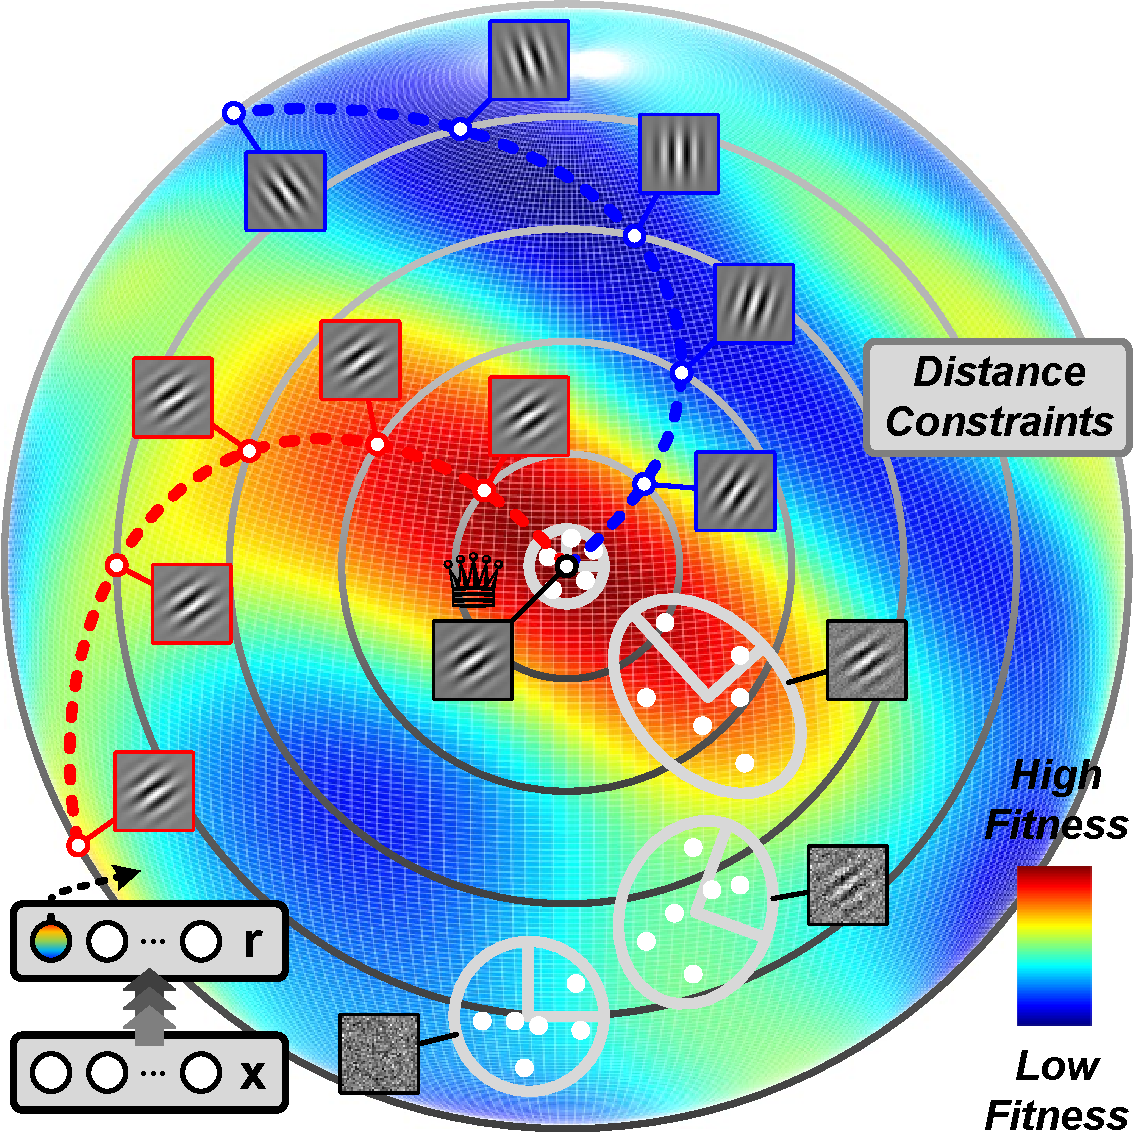
\includegraphics[width=0.5\textwidth]{Figs/methods.pdf} 
\caption{
{\bf Visualization of numerical optimization procedures.} Spherical constraint: solution space of the stimulus with energy constraint $\left\| x \right\| = 1$, an $N$ dimensional sphere centered on the origin. Optimal stimulus search trajectory: best solutions (patterns with black frame boarders) from sequential search iterations with adaptive landscape modeling (gray eclipses with varying diameters); visualization following \cite{muller2010black}. Distance constraints (gray circles): solution spaces of stimuli with $0.1\pi$ to $0.5\pi$ distances from the optimal stimulus. Invariance path (dashed red curve): solutions of the invariance path searches. Selectivity path (dashed blue curve): solutions of the selectivity path searches. Target neuron in this visualization is optimally tuned to a $45^{\circ}$ Gabor pattern, invariant to phase changes, and selective to orientation changes.}
\label{fig:methods}
\end{figure}

In this work, a unit's ``optimal stimulus'' was numerically derived through the iterative optimization as \begin{equation} \label{eq:O1} \hat{x} = \underset{x} {\arg\max} f\left(x\right) = \underset{x_{g} \in \Omega \left( x_{g-1} , m_{g-1} \right)}{\arg\max} f\left(x_{g}\right),\end{equation} where $m_{g}=U\left(\left\lbrace f\left(x_{g}\right) \right\rbrace , m_{g-1}\right)$ and $1 \le g \le G$, subject to $\left\| x \right\| = 1$.  
We note that there is no general guarantee that an optimum found by this procedure will be a global optimum; however, we argue that even exploring the response landscape around a high local maximum is useful in characterizing a unit.
The algorithm started from random initial point $x_{0}$ on an $N$ dimensional sphere (e.g. the noise pattern shown in the bottom of Fig.~\ref{fig:methods}) and samples from set of $\lambda$ neighboring points (through evaluation of the function $\Omega$) were taken as candidates to be evaluated, from an initial model $m_{0}$ with null distribution (in this work, multivariate Gaussian distribution starting with covariance matrix $\Sigma = I$). 
By measuring the response magnitude (``fitness,'' in the nomenclature of derivative-free optimization) of sampled points $\left\lbrace f\left(x_{g}\right) \right\rbrace$, the algorithm updates its model $m_{g}$ (i.e.~mean and covariance of the distribution, through function $U$) for generating samples in the following iterations, where the same operations repeat.
% why is this parameter given a name?  Is it useful to know that?
We set a threshold on the maximum allowed number of iterations, $G$, to prevent the algorithm from running for an unreasonably long time; however, more frequently, early termination occurred when the sample neighborhood size shrank below threshold, as shown in the center of Fig.~\ref{fig:methods}. Though the fitness landscape can be highly nonlinear, such sequential optimization procedure is often capable of gradually accumulating knowledge of the landscape and adjusting its search directions to climb onto higher fitness areas, and the smoother the landscape is, the faster the algorithm converges. As exemplified in Fig.~\ref{fig:methods}, the ``most salient pattern'', or direction leading to high fitness areas usually can be rapidly extracted (see Fig.~\ref{fig:ind_res} for more examples). In most scenarios, fixing the maximally allowed number of fitness evaluations $\lambda G$ to, e.g., $100N$ (as adopted for the optimal stimulus search in this work) can lead to reasonably good convergence speed vs.~quality trade-off. The aforementioned sequential optimization concept is in fact commonly adopted in modern stochastic optimization \cite{spall2005introduction}, and the CMA-ES (Covariance Matrix Adaptation Evolution Strategy) algorithm \cite{hansen2001completely} is chosen as the back-end solver of this numerical framework, for its good convergence speed and capability of handling ``rugged'' response landscapes. Readers can refer to \cite{hansen2001completely} for detailed definitions of model $m$ and functions $\Omega$ and $U$.
The energy constraint on the stimulus search space was implemented by simply navigating the stimulus space in spherical coordinates, with a fixed radius.
%through a spherical projection before evaluation, i.e.~$f\left(p_s\left(x\right)\right)$ where $p_{s}\left(x\right) = {x} / {\left\|x\right\|}$, while the solver worked in an unconstrained manner.

In order to analyze the results of optimal stimulus searches, we adopted the following measures: (1) \emph{Spectral complexity}, which is estimated through the $L^{1}$ norm of the (2 dimensional) Fourier power spectrum of optimal stimulus, i.e.~$\left\| \mathcal{F}(\hat{x}) \right\|_{1}$, where higher value suggests higher non-sparsity (i.e.~more spectral components required to represent the signal). (2) \emph{Explanation power}, which is estimated as the mean of the linear explainability of task-related stimuli---rectified inner-product distances between a set of $n$ task-related stimuli $\left\lbrace x^{t} \right\rbrace$ and the optimal stimulus itself, i.e.~$\frac{1}{n}\sum_{i=1}^{n}\max\left(\langle x^{t}_{i} , \hat{x} \rangle , 0\right)$---and measures how well the optimal stimulus can linearly ``approximate'' task-related stimuli (or intuitively how much neuronal response might be elicited). (3) \emph{Encoding specificity}, which utilizes the optimal stimulus search as an inverse function $f^{-1}$ of a representation $r$ (i.e.~searching for the optimal stimulus of an imaginary neuron, as shown in Fig.~\ref{fig:concept}, tuned to the representation of a reference stimulus) and measures the average of structural similarities (SSIM) \cite{wang2004image} between task-related reference stimulus $x^{*}$ and $n$ reconstructed stimuli (with randomized initializations), i.e.~$\frac{1}{n}\sum_{i=1}^{n} \mathrm{SSIM}\left(x^{*} , \hat{x}^{*}_{i} \right)$ where \begin{equation} \label{eq:O2} \hat{x}^{*} = \underset{x}{\arg\max} \left( e^{-\left\|f\left(x\right)-r\right\|} \right) \end{equation} and $r = f\left(x^{*}\right)$, indicating how specific (or non-confounding) a representation $r$ is encoded.

%\underset{x}{\arg\max} f^*\left(x\right)
% ssim human vision similarity

\subsection*{Quasi-Second-Order Characterization: Invariance and Selectivity Path Search and Analysis}

\begin{figure}
\centering 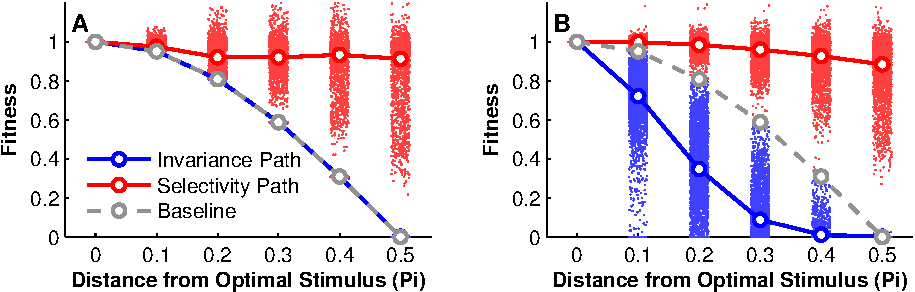
\includegraphics[width=0.5\textwidth]{Figs/fda.pdf} 
\caption{
{\bf Fitness-distance diagram.} Invariance (red) and selectivity (blue) curves: fitnesses of invariance and selectivity path search results plotted against distances from the optimal stimulus. Baseline (dashed gray) curve: graph of cosine function; invariance and selectivity curves of single inner-product neuron. Subsequent analyses, including path potential, subspace capacity and subspace alignment, can be performed. Invariance and selectivity path potentials can be defined on either the arccosine normalized diagram (shaded red and blue areas), or on the original diagram (line integrals).}
\label{fig:fd_diag}
\end{figure}

%\underset{x_{\delta}}{\arg\max} \hat{f}\left(x_{\delta}\right)

While the optimal stimulus provides important information about the nature of units in a network, important additional information can be extracted about the response landscape around the peak response.  The begin to quantify properties of this landscape, we define the ``selectivity'' and ``invariance'' paths.

With respect to the optimal stimulus $\hat{x}$, the searches of invariance and selectivity paths, which consist of sets of invariant stimuli ($\left\lbrace x^{+}_{\delta} \right\rbrace$, i.e.~optimally excitatory) and selective stimuli ($\left\lbrace x^{-}_{\delta} \right\rbrace$, i.e.~optimally inhibitory) respectively, are formulated as
\begin{align}
x^{+}_{\delta} &= \underset{x_{\delta}}{\arg\max} f\left(x_{\delta}\right) \label{eq:I1} \\
&= \underset{x_{\delta}}{\arg\max} \left( e^{-\left\|f\left(x_{\delta}\right)-f\left(\hat{x}\right)\right\|} \right); \label{eq:I2} \\
x^{-}_{\delta} &= \underset{x_{\delta}}{\arg\min} f\left(x_{\delta}\right) \label{eq:S1} \\
&= \underset{x_{\delta}}{\arg\min} \left( e^{-\left\|f\left(x_{\delta}\right)-f\left(\hat{x}\right)\right\|} \right); \label{eq:S2}
\end{align}
where $0 < \delta \le \frac{\pi}{2}$, subject to $\left\| x_{\delta} \right\| = 1$ and $\langle x_{\delta} , \hat{x} \rangle = \cos\left(\delta\right)$. As visualized in Fig.~\ref{fig:methods}, the invariance path characterizes the $N$ dimensional ``curve'' that leads toward (or ideally maintains at) fitness as high as possible while moving away from the optimal stimulus, and the selectivity path characterizes the ``curve'' that leads toward fitness as low as possible while moving away. The search process was implemented as multiple runs of maximization/minimization on discretized $\delta \in \left\lbrace 0.1\pi, 0.2\pi, 0.3\pi, 0.4\pi, 0.5\pi\right\rbrace$, as the circular distance constraints shown in Fig.~\ref{fig:methods}, where each run is initialized with the result from previous run (and the $0.1\pi$ run directly with optimal stimulus $\hat{x}$) to increase the path continuity and searching speed. Each $\delta$ of both paths has a budget of $20N$ fitness evaluations which in this work appears to be practically sufficient. The maximization and minimization simply use the same back-end solver, and the linear constraint $\langle x_{\delta} , \hat{x} \rangle = \cos\left(\delta\right)$ can be easily handled through an extra conic projection before evaluation, i.e.~$f\left(p_c\left(p_s\left(x\right)\right)\right)$ where $p_c\left(x\right) = \cos\left(\delta\right)\hat{x} + \sin\left(\delta\right)\dot{x} \mathbin{/} \left\|\dot{x}\right\|$ and $\dot{x} = x - \langle\hat{x},x\rangle \hat{x}$. The way the simple linear constraint is constructed to enforce the exploration of a larger extent of the fitness landscape is the one of the main differences compared to \cite{erhan2010understanding}.
In this work, the distance constraint $\delta$ only goes up to $\frac{\pi}{2}$, since on the $N$ dimensional sphere, stimuli fall in $\frac{\pi}{2} < \delta \le \pi$ are simply ``negatives'' of those in $0 < \delta \le \frac{\pi}{2}$, which are of less uniqueness and interest; nevertheless, going up to the full range $0 < \delta \le \pi$ is numerically supported.

For analyzing the results of invariance/selectivity path searches, the following measures are adopted: (1) \emph{Path potential}: while the search results of invariance/selectivity paths can be visualized via the \emph{fitness-distance diagram} \cite{jones1995fitness} as shown in Fig.~\ref{fig:fd_diag} where perfect invariance and selectivity are flat lines at highest and lowest fitnesses respectively, the baselines of invariance and selectivity also can be intuitively (and analytically) defined as paths of the simplest form of neural networks---an inner-product neuron, $f(x) = w^{T}x$---which precisely overlap and follow the monotonic cosine falloff from its optimal stimulus $\hat{x}=w$, as $f(x_{\delta}) = \cos(x_{\delta})$ by definition; the invariance (and selectivity, similarly) path potential of a unit representation can thus be defined as $\int_{0}^{\frac{\pi}{2}}{\left| \cos^{-1}\left(f\left( x^{+}_{\delta} \right)\right) - \delta \right|}\mathrm{d}\delta \mathbin{/} {\frac{\pi}{2}}$, the area sandwiched between the invariance (and selectivity) and baseline curves (in $\cos^{-1}$ domain such that both potential values fall in the range $\left[0,1\right]$), measuring how invariant (and selective) a target neuron is compared to the baseline (i.e.~zero invariance/selectivity potential); for population representation where no baseline can be easily identified, the invariance (and selectivity) path potential is alternatively defined as $\int_{0}^{\frac{\pi}{2}}{\exp\left(-\left\|f\left(x^{+}_{\delta}\right)-f\left(\hat{x}\right)\right\|\right)}\mathrm{d}\delta \mathbin{/} {\frac{\pi}{2}}$. (2) \emph{Subspace capacity}: compared to path potential, which is designed to characterize the best invariance/selectivity path even when only one of such exists, subspace capacity estimates the ``dimensionality'' (i.e.~how diverse different paths can be) of the linear subspace formed by multiple path search results via the nuclear norm of concatenation of $n$ results $\left\|\left[x_{\delta,1},\dots,x_{\delta,n}\right]\right\|_{*}$ (in this work $n=20$ runs at $\delta=0.1\pi$). (3) \emph{Subspace alignment}, which measures the alignment between subspaces formed by task-related stimuli and invariance/selectivity paths (i.e.~how likely the invariance/selectivity can benefit, e.g., stimulus recognition) via estimating the sparsity of $n$ path search results projected onto the principal component vectors $V$ of task-related stimuli $\left\lbrace x^{t} \right\rbrace$, i.e.~$\frac{1}{n}\sum_{i=1}^{n} \left\| Vx_{\delta,i} \right\|_{1}$ ($n=20$ runs at $\delta=0.1\pi$ as well). %SUBSPACE OVERLAP?


\subsection{Deep Convolutional Networks}

The methods and measures proposed above were tested using random convolutional neural networks (``randnets,'' \cite{pinto2009high, sthor}), a simplified variety of a deep convolutional neural network \cite{fukushima1980neocognitron, lecun1998gradient, riesenhuber1999hierarchical, krizhevsky2012imagenet}, where convolution kernel weights are randomly assigned rather than trained.  While these models cannot match the performance of deep networks trained on very large quantities of data (e.g. using backpropagation, \ref{krizhevsky2012imagenet}), they are suprisingly competitive for a variety of tasks, especially in the regime where massive quantities of training data are not available \cite{pinto2009high, cox2011beyond, viglarge}.  Importantly, they do not require extensive training---a classifier is trained on the output of the network, but the weights of the network itself are not trained---meaning that large numbers of candidate networks can be rapidly generated with different hyperparameters (e.g. different kernel sizes, normalization exponents, etc.) and compared.  Thus, random networks are a useful tool when exploring a diversity of network architectures in settings where absolute task performance is not essentail.  We have previously shown that searching within the space of hyperparamters can yield suprisingly effective networks, even when the networks are not trained in the conventional sense \cite{james}.

The random networks used here were implemented using the open source STHOR library \cite{sthor}.
Reference code for the experiments described in this paper is available at [URL TBD].  As with other convolutional networks, our networks consist of a standard cascade of convolution, nonlinear activation, pooling, and normalization layers (which together define a single ``level'' in this work).  In this work, we focused 100 shallow networks (i.e.~one-level, ``L1,'' models) and 100 deep networks (i.e.~two-level, ``L2,'' models) were randomly generated (all with 32 top-layer neurons) and tested to see how their representations vary with networks' depths and affect networks' performances (as shown in Fig.~\SFpef{}) on face pair matching tasks---accuracy of identifying pairs of different pictures from the same person and rejecting those from different persons---against the Labeled Faced in the Wild (LFW/LFW-a) dataset \cite{LFWTech, wolf2011effective}. Stimulus dimensionalities of shallow and deep neurons are $N=121$ and $N=441$ (i.e.~$11\times11$ and $21\times21$ receptive field sizes) respectively.


